\chapter[Metodologia]{Metodologia}
\label{chap:metodologia}

\section{Imagens}
\label{sec:imagens}

Para realização da atividade proposta, foram utilizadas 4 imagens escolhidas aleatoriamente no portal pexels.com, conforme Figura \ref{imagens-rgb}.

\begin{figure}[!htpb]
 \centering
 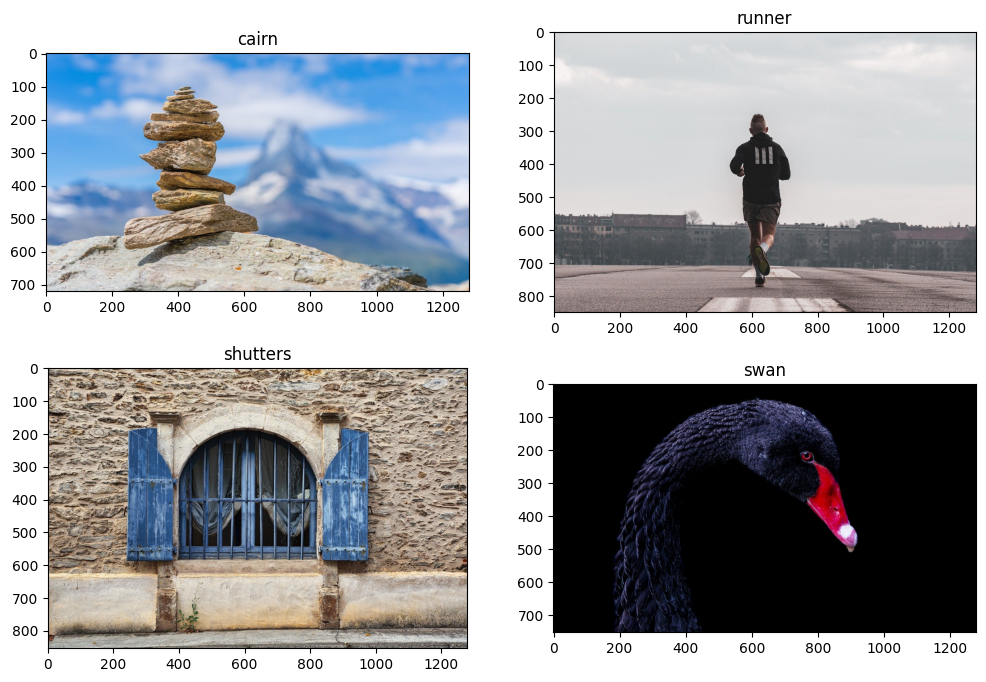
\includegraphics[scale=0.5]{Elementos/Figuras/metodologia-originais-rgb.png}
 \caption{Imagens em RGB}
 \label{imagens-rgb}
\end{figure}

As imagens selecionadas foram pré-processadas e transformadas em escala de cinza, conforme apresentadas na Figura \ref{imagens-gray}, para viabilização das transformações propostas e análise dos resultados obtidos.

\begin{figure}[!htpb]
 \centering
 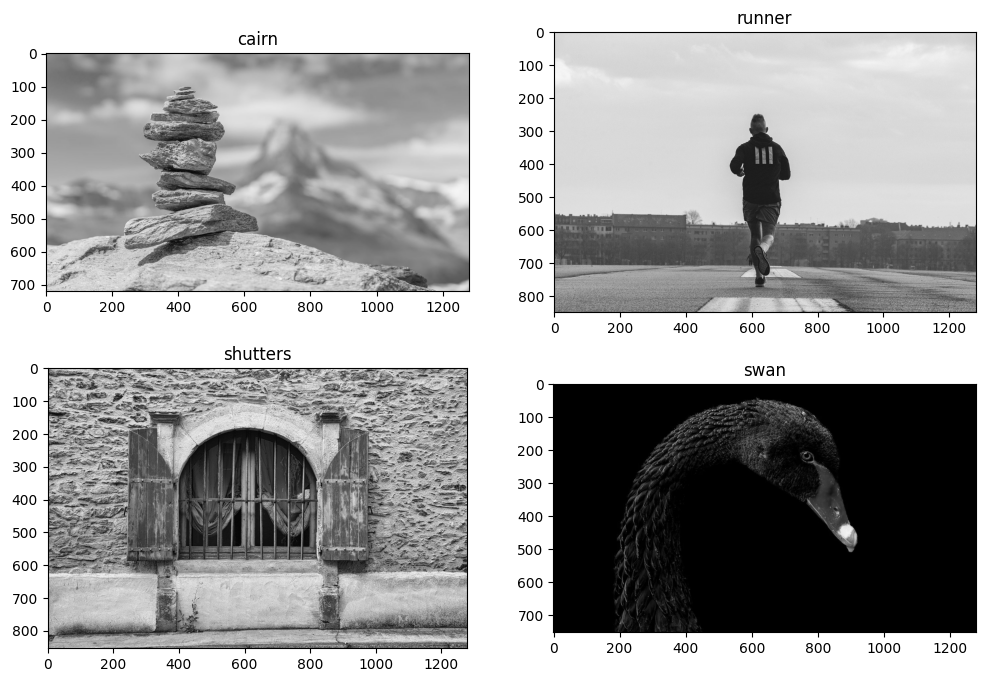
\includegraphics[scale=0.5]{Elementos/Figuras/imagens-originais-gray.png}
 \caption{Imagens em escala de cinza}
 \label{imagens-gray}
\end{figure}

Para um melhor entendimento e interpretação dos resultados, tendo como linha de base as características pertinentes às imagens originais, foram extraídas as informações espaciais das imagens em escala de cinza e exibidas na Figura \ref{imagens-si}: desvio padrão e as imagens resultantes da aplicação do Filtro de \textit{Sobel}.

\begin{figure}[!htpb]
 \centering
 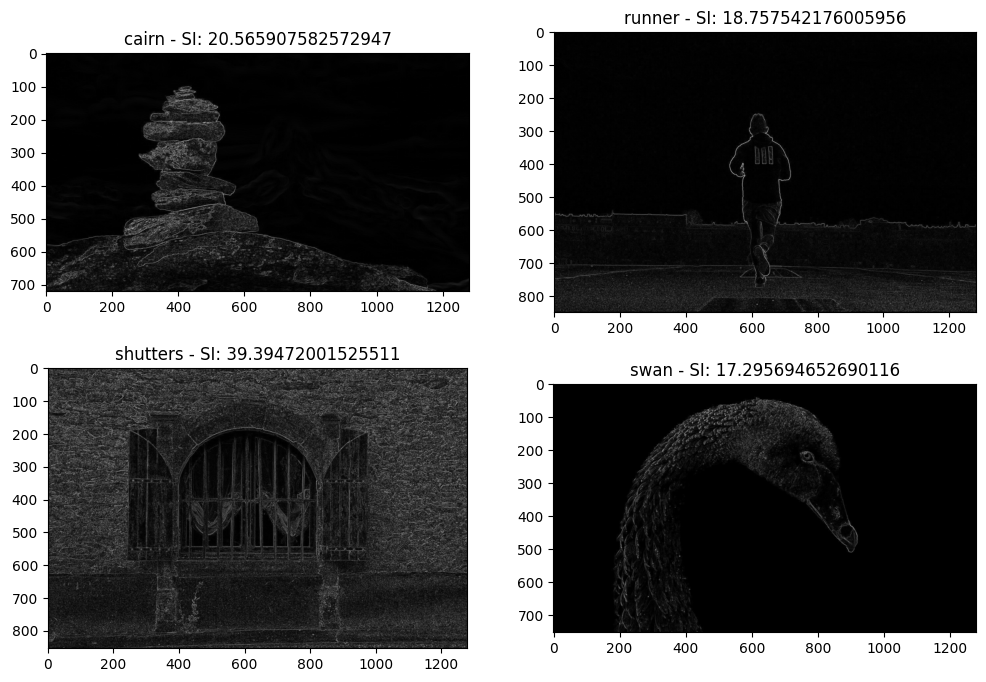
\includegraphics[scale=0.5]{Elementos/Figuras/metodologia-si.png}
 \caption{Imagens resultantes da aplicação do filtro de \textit{Sobel} com as respectivas Informações Espaciais (SI)}
 \label{imagens-si}
\end{figure}

\section{Recursos Computacionais}
\label{sec:recursos}

Para a realização desta atividade avaliativa, foi utilizado o ambiente de desenvolvimento colaborativo \textit{Google Colab} (Figura \ref{imagens-colab}). A linguagem de programação adotada foi \textit{Python} e as bibliotecas especializadas utilizadas neste trabalho de acordo suas aplicações, foram:

\begin{itemize}
    \item \textbf{OpenCV} (cv2) - Manipulação e processamento das imagens;
    \item \textbf{NumPy} (numpy) - Funções matemáticas e operações com vetores e matrizes;
    \item \textbf{scikit-image} (skimage) - Processamento das métricas dos resultados;
    \item \textbf{os} (os) - Interação com o sistema operacional no que tange a manipulação dos arquivos de imagens armazenados no sistema de arquivos;
    \item \textbf{Matplotlib} (matplotlib) - Criação dos gráficos e visualização das imagens e dados.
\end{itemize}


\begin{figure}[!htpb]
 \centering
 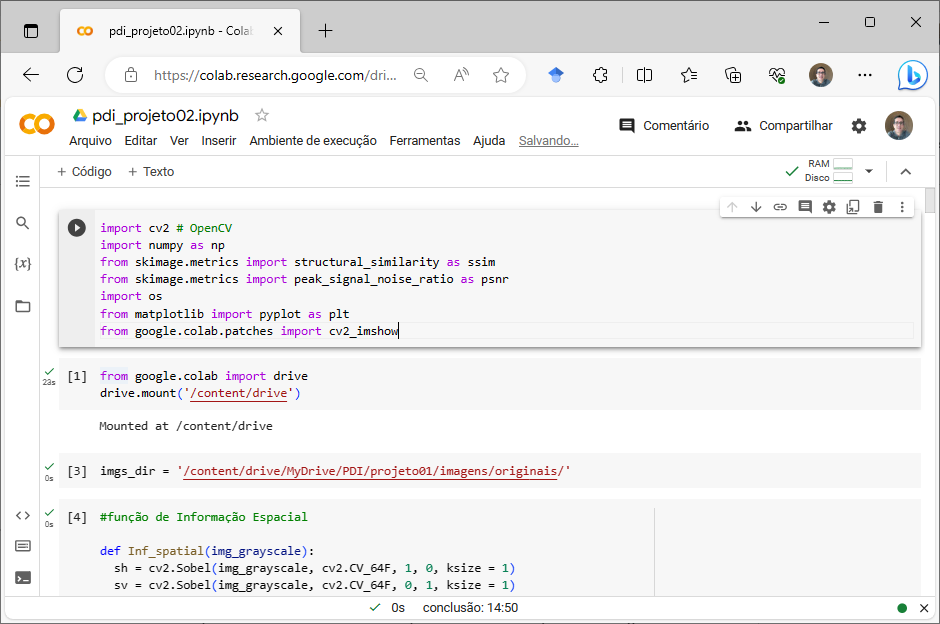
\includegraphics[scale=0.5]{Elementos/Figuras/metodologia-colab.png}
 \caption{Tela do ambiente \textit{Google Colab})}
 \label{imagens-colab}
\end{figure}
